% !TeX root = ../UrrutiaAnguiano_CandidaturaDefensa.tex
% !TeX spellcheck = es_MX 


\section{Teorías de esparcimiento múltiple y técnicas de medición}
\subsection{Modelo de esparcimiento coherente}

{\setbeamertemplate{frametitle}[centertitle]{}
\begin{frame}{\underline{Teoría de esparcimeinto múltiple\footnotemark[1]}}
	{Jerarquización de Foldy-Lax}
	\centering
\begin{columns}
	\column{.9\squeezetwo}
	\begin{block}{\centering N esparcidores}
		\centering
		\begin{tasks}(2)
			\task Iluminados con onda plana
			\task $N\to \infty$ ecuaciones
			\task $V:$ Volumen semiinfinito
			\task $\rho(\vb{R})$
		\end{tasks}
		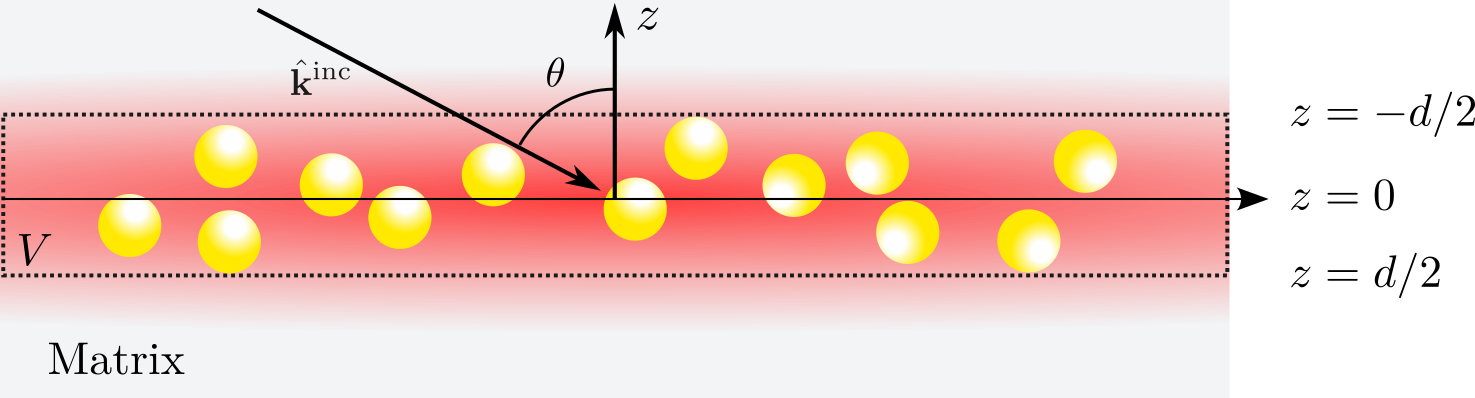
\includegraphics[scale = 1]{img/1-CSM/Fig-CSM.png}
	\end{block}
	\column{.9\squeezetwo}
	
		\begin{align*}
		\vb{E}^\text{exc}_k(\vb{r}) = & 
			\vb{E}^\text{inc}(\vb{r}) + \sum_{\ell\neq k}^N \vb{E}^\text{ind}_\ell(\vb{r})\\
		\vb{E}^\text{ind}_\ell(\vb{r}) = & 
			\int\dd^3 r' \mathbb{G}(\vb{r},\vb{r}') \times
			\int\dd^3 r''\mathbb{T}(\vb{r}'-\vb{r}_\ell,\vb{r}''-\vb{r}_\ell) \vb{E}_\ell^\text{exc}(\vb{r}'')\\
		\textcolor{sblueFC}{\langle\vb{E}(\vb{r})\rangle =} 
			& \textcolor{sblueFC}{\vb{E}^\text{inc}(\vb{r}) +  \sum_{\ell = 1}^N 
				\underbrace{\left(\prod_{k = 1}^N \int\dd^3 r_k \rho(\vb{R}) \vb{E}^\text{ind}_\ell(\vb{r})\right)}_{\text{\normalsize $\langle \vb{E}_\ell^\text{ind}\rangle$}}}
		\end{align*}

\end{columns}
\vskip1em
\begin{columns}
	\column{.9\squeezetwo}
	\begin{alertblock}{Aproximación de esparcidor individual (SSA)}
		\begin{align*}
                        \langle \vb{E}^\text{ind}_\ell(\vb{r}) \rangle =& \int\dd^3 r'\mathbb{G}(\vb{r},\vb{r}')
                            \int\dd^3 r'' \times\\
                            & \int \dd^3 r_\ell \rho(\vb{r}_\ell) \mathbb{T}(\vb{r}'-\vb{r}_\ell,\vb{r}''-\vb{r}_\ell)
								\langle \vb{E}_\ell^\text{exc}(\vb{r}'',\vb{R})\rangle_\ell\\
		\langle \vb{E}_\ell^\text{exc}(\vb{r}'',\vb{R})\rangle_\ell
					=& \prod_{\substack{k =1 \\ k\neq \ell}}^N  \int\dd^3 r_k \rho(\vb{R}|\vb{r}_\ell) \vb{E}^\text{exc}_\ell(\vb{r}'')
\uncover<2->{ \textcolor{sredFC}{ = \vb{E}^\text{inc}(\vb{r}'')}}					
		\end{align*}
	\end{alertblock}
	\column{.9\squeezetwo}
	\begin{alertblock}{Aproximación Cuasicristalina (QCA)}
	\begin{align*}
		\langle \vb{E}_\ell^\text{exc}(\vb{r}'',\vb{R})\rangle_\ell =& \vb{E}^\text{inc}(\vb{r}'')
		+ \sum_{\substack{m =1 \\ m\neq \ell}}^N  \int\dd^3 r' \mathbb{G}(\vb{r}',\vb{r}'') \times \notag\\
		& \int\dd^3 r'''\int \dd^3 r_m \rho(\vb{r}_m) \mathbb{T}(\vb{r}'-\vb{r}_m,\vb{r}'''-\vb{r}_m) \langle \vb{E}_m^\text{exc}(\vb{r}'',\vb{R})\rangle_{\ell,m}\\
		\langle \vb{E}_m^\text{exc}(\vb{r}'',\vb{R})\rangle_{\ell,m},
		&= \prod_{\substack{n =1 \\ n\neq \ell,m}}^N  \int\dd^3 r_n \rho(\vb{R}|\vb{r}_\ell,\vb{r}_m) \vb{E}^\text{exc}_n(\vb{r}'')
\uncover<2->{\textcolor{sredFC}{ = \langle \vb{E}_\ell^\text{exc}(\vb{r}'',\vb{R})\rangle_\ell}}
	\end{align*}
\end{alertblock}
\end{columns}	% 

\begin{textblock*}{80mm}(145mm,137.5mm)
	\begin{flushleft}
		\scriptsize
		\rule{30mm}{.5pt}\\
		\footnotemark[1]\fullcite{garcia2012multiple}
	\end{flushleft}
\end{textblock*}
\end{frame}
}

% --------------------------------------------------------------
\begin{frame}[t]{\underline{Modelo de esparcimiento coherente (CSM)}}
				{Caso monodisperso\footnotemark[1]}
	\centering
\begin{columns}
	\column{.9\squeezetwo}
	\begin{block}{\centering N esparcidores}
		\centering
		\begin{tasks}(2)
            \task QCA
			\task Esferas de radio $a$
			\task Película de grosor $d\to 0$
			\task $\rho(\vb{r}_\ell) = 1/V$
			\task Correlación de esfera dura
			\task $\alpha = 2\Theta /[(ka)^2 \cos\theta]$
		\end{tasks}
		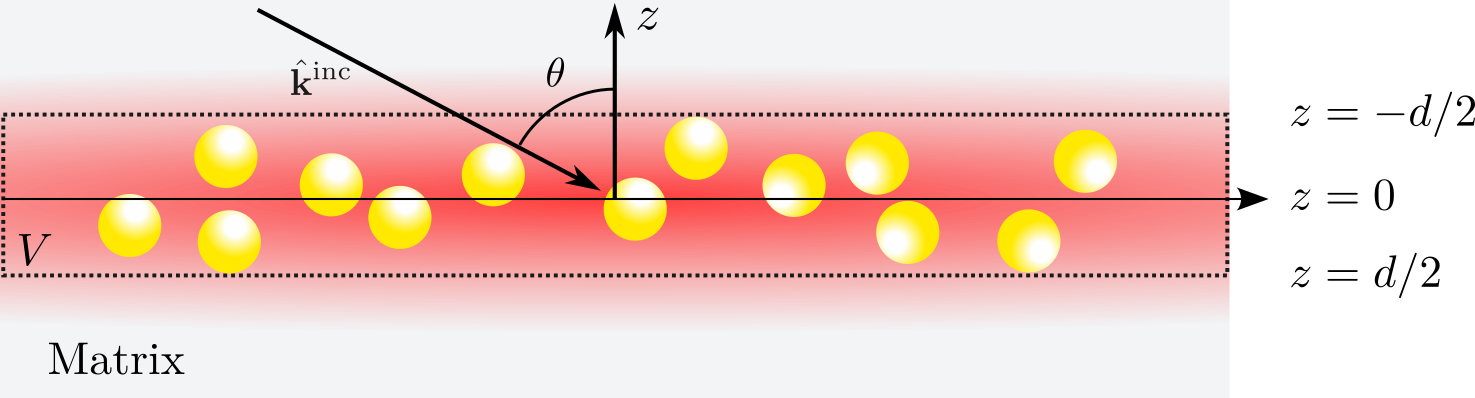
\includegraphics[scale = 1]{img/1-CSM/Fig-CSM.png}
	\end{block}
	\column{\squeezetwo}
	\begin{align*}
		\langle \vb{E}_\text{SSA}^\text{ind}(\vb{r})\rangle &=
		\begin{dcases}
			-\alpha  S_i(\pi-2\theta)	\exp(i\vb{k}^\text{r}_\text{coh}\cdot\vb{r}) \vb{E}^\text{inc}, & z > 0 \\
			-\alpha S(0)\exp(i\vb{k}^\text{t}_\text{coh}\cdot\vb{r}) \vb{E}^\text{inc},  & z < 0 \\
		\end{dcases}
	\end{align*}
	\begin{align*}
			\langle\vb{E}^\text{exc}_\ell(\vb{r}) \rangle_\ell &=
		\vb{E}^\text{exc}_\text{r}(\vb{r})\ \exp(i\vb{k}^\text{r}_\text{coh}\cdot\vb{r}) +
		\vb{E}^\text{exc}_\text{t}(\vb{r})\ \exp(i\vb{k}^\text{t}_\text{coh}\cdot\vb{r})\\
		\langle \vb{E}_\text{QCA}^\text{ind}(\vb{r})\rangle &=
		\begin{dcases}
			-\alpha \bigg( S_j(0) \norm{\vb{E}^\text{exc}_\text{r}(\vb{r})} +  S(\pi-2\theta)\norm{\vb{E}^\text{exc}_\text{t}(\vb{r})}\bigg)
			\exp(i\vb{k}^\text{r}_\text{coh}\cdot\vb{r}) \vu{E}^\text{inc}, & z > 0 \\
			-\alpha \bigg( S_j(\pi-2\theta) \norm{\vb{E}^\text{exc}_\text{r}(\vb{r})} + S(0)\norm{\vb{E}^\text{exc}_\text{t}(\vb{r})}\bigg)
			\exp(i\vb{k}^\text{t}_\text{coh}\cdot\vb{r}) \vu{E}^\text{inc},  & z < 0 \\
		\end{dcases}\\
		\vb{E}^\text{exc}_\text{r}(\vb{r}) &= -\frac{\alpha}{2} \bigg( S_j(0) \norm{\vb{E}^\text{exc}_\text{r}(\vb{r})} +  S(\pi-2\theta)\norm{\vb{E}^\text{exc}_\text{t}(\vb{r})}\bigg) \vu{E}^\text{inc},
		\\
		\vb{E}^\text{exc}_\text{t}(\vb{r}) &= \vb{E}^\text{inc}(\vb{r}) -\frac{\alpha}{2} \bigg( S_j(\pi-2\theta) \norm{\vb{E}^\text{exc}_\text{r}} + S(0)\norm{\vb{E}^\text{exc}_\text{t}(\vb{r})} \bigg)
	\vu{E}^\text{inc}.
	\end{align*}
\end{columns}


\begin{tikzpicture}[node distance=20 mm and 50mm]
    \path (0,0) node [concept]  (meta) {\Large Coeficiente de reflexión y transmisión};
    
    \node[below of=meta] (eqs){
         \begin{minipage}{80mm}
         \begin{align*}
         	r^{(j)}_\text{CSM}(\theta)&=\frac{-\alpha S_j(\pi-2\theta)}
				{1+\alpha S(0)+\frac14 \alpha^2 \left[S^2(0)-S_j^2 (\pi-2\theta) \right]}\\
			t^{(j)}_\text{CSM}(\theta)&=\frac{1-\frac14\alpha^2\qty[S^2(0)-S_j^2(\pi-2\theta)]}
				{1+\alpha S(0)+\frac14 \alpha^2 \left[S^2(0)-S_j^2 (\pi-2\theta) \right]}
         \end{align*}
         \end{minipage} };
     
     \node [flowbox, right=of eqs] (sus) {\fbtitle{Presencia de sustrato (Reflexión)}
     	\nodepart{two}
     	\begin{minipage}{80mm}
     		\begin{align*}
     			r^{(j)}(\theta_i)&= \frac{r_\text{sm}^{(j)}(\theta_i) + r_\text{CSM}^{(j)}(\theta_t)}
										 {1+r_\text{sm}^{(j)}(\theta_i) r_\text{CSM}^{(j)}(\theta_t)}
     		\end{align*}
     	\end{minipage}};
     
    \draw[hidden] (eqs.east) -- 
    			node[above,text=sdgrayFC,font=\itshape\scriptsize,anchor=south] {Múltiples reflexiones}
    			(sus.west);
\end{tikzpicture}

\begin{textblock*}{80mm}(145mm,137.5mm)
	\begin{flushleft}
		\scriptsize
		\rule{30mm}{.5pt}\\
		\footnotemark[1]\fullcite{garcia2012multiple}
	\end{flushleft}
\end{textblock*}

\end{frame}

%
%
\begin{frame}{\underline{Modelo de esparcimiento coherente (CSM)}}
			{Caso monodisperso\footnotemark[1] y caso polidisperso\footnotemark[2]}
%
\begin{center}
    \begin{tikzpicture}[node distance=20mm and 80mm]
%%
%%    % mono
        \path (0,0) node[concept,align=center] (mono) {CSM};
        \node[below=of mono,yshift=0cm, font=\small] (campo) {%
            \begin{minipage}{100mm}
                \begin{align*}
					\langle \vb{E}_\text{QCA}^\text{ind}(\vb{r})\rangle =
					\begin{dcases}
						-\alpha \bigg( S_j(0) \norm{\vb{E}^\text{exc}_\text{r}(\vb{r})} +  S(\pi-2\theta)\norm{\vb{E}^\text{exc}_\text{t}(\vb{r})}\bigg)
							\exp(i\vb{k}^\text{r}_\text{coh}\cdot\vb{r}) \vu{E}^\text{inc}, & z > 0 \\
	 					-\alpha \bigg( S_j(\pi-2\theta) \norm{\vb{E}^\text{exc}_\text{r}(\vb{r})} + S(0)\norm{\vb{E}^\text{exc}_\text{t}(\vb{r})}\bigg)
							\exp(i\vb{k}^\text{t}_\text{coh}\cdot\vb{r}) \vu{E}^\text{inc},  & z < 0 \\
					\end{dcases}
    			\end{align*}
            \end{minipage}};
%%
        \node[flowbox, right=of mono] (rCSM) {\fbtitle{CSM monodisperso}
         \nodepart{two}
            \begin{minipage}{60mm}
                \begin{align*}
                r^{(j)}_\text{CSM}(\theta)&=\frac{-\alpha S_j(\pi-2\theta)}
					{1+\alpha S(0)+\dfrac14 \alpha^2 \left[S^2(0)-S_j^2 (\pi-2\theta) \right]}
    			\end{align*}
            \end{minipage}};
        
        \node[flowbox, fb-highlight, below=of rCSM, yshift=-40mm] (poli) {\fbtitle{CSM polidisperso}
		\nodepart{two}
		\begin{minipage}{60mm}
			\begin{align*}
				r^{(j)}_\text{CSM}(\theta)&=\frac{-\beta_+^{(j)}(\theta)}
				{1+\beta_F+\dfrac14 \left[ \beta_F^2 - \beta_+^{(j)} (\theta)\beta_-^{(j)}(\theta)\right]}
			\end{align*}
		\end{minipage}};

        \draw[conn] (mono) -- (campo);
        \draw[conn] (campo.east) -| (rCSM.south);

        \draw[connr] (mono.east) -| (campo.15)
                      node[right,near end, text=sredFC ,anchor=west,yshift=0cm] {
                \begin{minipage}{20mm}
                    \begin{align*}
                        \int\dd{a}\rho(a)
                    \end{align*}
                \end{minipage}};

        \draw[connr] (campo.345) |- (poli.west)
            node[left,near start, anchor=east, text=sredFC, yshift=-15mm] {
                \begin{minipage}{60mm}
                \begin{align*}
                    \beta_F(\theta) = \eta \int_{0}^{\infty} \rho(a)S(0)\dd{a}&\\
					\beta_{\pm}^{(j)}(\theta) = \eta \int_{0}^{\infty} \rho (a)S_{j}(\pi-2\theta)\exp(\pm2ik_z^\text{inc} a)\dd{a}&\\
					\eta = \dfrac{2 \Theta}{(ka_0)^2 \cos\theta}&
                \end{align*}
                \end{minipage}};
    \end{tikzpicture}
    \end{center}
%
%\begin{textblock*}{80mm}(145mm,137.5mm)
%	\begin{flushleft}
%    \scriptsize
%	\rule{30mm{.5pt}\\
%	\footnotemark[1]\fullcite{garcia2012multiple}
%	\footnotemark[2]\fullcite{vazquez-estrada_optical_2014}
%	\end{flushleft}
%\end{textblock*}
\end{frame}

